\documentclass{llncs}
%
%-- coding: UTF-8 --
\usepackage[UTF8]{ctex}
\usepackage{amsfonts}
\usepackage{amstext}
\usepackage{amsmath}
\usepackage{enumitem}
\usepackage{multirow}
\usepackage{graphicx}
\usepackage[center]{subfigure}
\usepackage{amssymb}
\usepackage{graphicx,amsmath} % Add all your packages here
\usepackage{subfigure}
\usepackage{algorithm}
\usepackage{algorithmic}
\renewcommand{\algorithmicrequire}{ \textbf{Input:}}
\renewcommand{\algorithmicensure}{ \textbf{Output:}}
\usepackage{url}
\usepackage{cite}
\usepackage{color}

\usepackage{makecell}
\usepackage{booktabs}
%
\begin{document}
	
\title{基于多任务学习的商业选址推荐方法的研究}
\author{陈麒先}
\institute{北京航空航天大学,计算机学院}
\maketitle

\begin{abstract}
商业选址是一类重要的投资决策问题。其重要性主要体现在投资的长期性、固定性以及对经济效益的决定性上。在传统的商业选址问题中,通常的考量因素往往涵盖了地域、交通、竞争压力以及人流量等方面。在这种情况下,投资者的经验以及数据信息来源的有效性将起到决定性的作用。随着移动互联网时代的到来,越来越多的商业应用,如美团、大众点评等渐渐走入人们的生活。这其中蕴含着巨大潜在的商业价值有待挖掘,尤其对于商业选址这类重要的问题而言,数据所提供的参考信息已然成为大数据时代的选址利器。

为此,本文对深度多任务机器学习模型在商业选址推荐方面的应用进行了考察和研究。通过对多个商业选址的多个决定因素进行分析,并对使用多任务学习在商业领域的应用情况进行了综述。从大众点评的用户评论中采集到的大量用户评论数据表明,通过提取出与商场有关的内部与外部特征,应用关联特征的深度多任务学习框架(Deep Multi-task Learning framework with Relational Attention, DMLRA),给出连锁品牌的投资预测是一种可行的商业选址问题解决方案。基于该模型运行的结果,可以有效地为投资者提供若干最优的决策方案。本文也通过对文献中提及大量具体案例进行实验探究,验证了模型实施的可行性与有效性,以保证商业选址的推荐方法能在真正投入到生产实践中后能在最大程度上为投资者带来经济效益。

此外,本文通过研究发现,对于一个有效的商业选址推荐平台而言,需要综合考量时间与位置信息、消费者行为与心理学信息、舆情评论信息等。选址过程中需要深入商圈细节,从而达到进行辅助选址的作用,并将体量庞大却联系较弱的海量数据从宏观角度综合演绎,无论是从经营策略、广告投放还是选址优化设计方面,都将为投资者提供敏锐的预测。在本文的最后,对采用多任务学习进行商业选址预测的工作进行总结,给出相关领域未来的发展前景预期,为相关研究提供辅助性的参考。

\keywords{多任务学习, 商业选址推荐, 综述}
\end{abstract}

\section{引言}
随着各种电子商务平台的日益兴盛,互联网每天都会产生大量的用户数据。这些丰富的用户数据资源与地理信息资源POI,对商业选址都会提供强有力的数据支持。而目前大多数的商业选址研究更多地采用传统的机器学习与数据挖掘方法,来进行商业投资位置的选择。

然而,尽管近年来机器学习领域已经取得了突破性的进展,但对于预测商业选址的准确度方面,仍存在一定的技术瓶颈。
首先,商业选址的成功判定标准涉及到多维度特征的提取,这是传统机器学习模型难以处理的~\cite{ZhouLiuCai}。
其次,不同的判定标准之间的相关性通常是复杂且无法预知的。
此外,商店特征与投资成功率之间的映射关系对于传统方法而言也是十分棘手的问题。由此构成了我们将多任务学习模型应用到商业选址问题的研究动机。

传统的商业推荐算法还存在其他一些问题,如数据来源来自调查问卷,或店铺的历史运营数据;优化目标多以最大化店铺的覆盖面积作为目标~\cite{jou2016deep};推荐方案更多地依赖于决策者经验和传统的运筹学方法,等等。

本文的目的在于,对文献中提及的数据组织和管理方法,以及多任务学习模型在商业选址问题的应用进行综述,使得推荐方案能够最大限度地,接近选址推荐的目标。
由于商业选址是一类十分宽泛的问题,因而在本综述文章中,将选址推荐的目标聚焦于连锁店与连锁品牌的选址推荐。
\begin{figure}
	\centering
	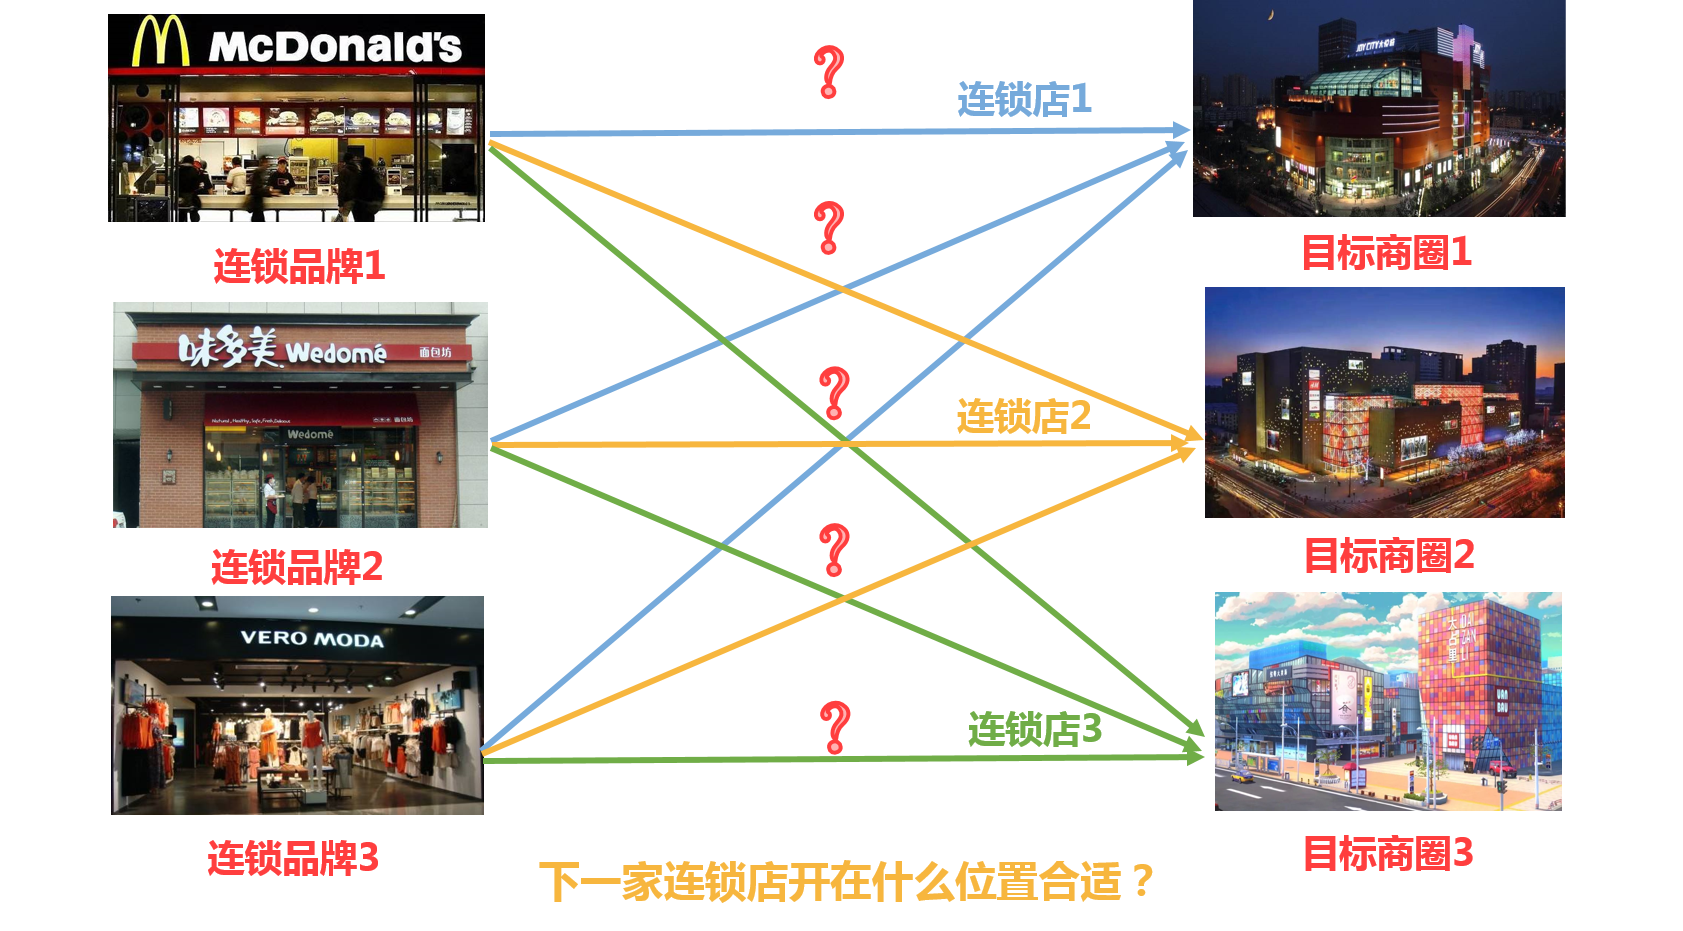
\includegraphics[width=0.8\columnwidth]{figures/intro.png}
	%  \setlength{\abovecaptionskip}{0pt}
	%  \setlength{\belowcaptionskip}{-20pt}
	\caption{问题描述}
	\label{intro}
\end{figure}

连锁店,是指若干共用同样的品牌名称,有统一的经营管理和商业运营标准,并分布于不同地理位置的一些店铺的总称~\cite{DongHongAn}。近年来,随着社会经济的持续发展和企业的不断扩张,连锁店的经营模式得到了更为广泛的应用。如餐饮业的海底捞火锅店、麦当劳、星巴克,服饰业的H\&M、Nike、Zara等品牌的迅猛发展,连锁店这种商业模式开始逐渐在市场中占据主导地位。由此为这些连锁品牌带来一个关乎企业发展的核心问题,即连锁店的选址问题。因此有必要对海量的用户产生数据进行分析,从而为投资者给出最优化的选址推荐。


\section{研究现状}
\subsection{商业选址的研究方法}
在商业选址方面,既有的研究成果主要利用了丰富的地理信息和社交媒体数据,对商业选址成功率给出具体预测结果。由于智能手机逐渐被大多数人使用,和GPS、北斗导航定位技术的普及,商业选址的数据来源也得到了极大的丰富~\cite{zhao2017mining,chen2017mining}。

在一些文献中,作者通过对商店地理位置数据,使用一种基于位置的社交网络,成功地预测了商店每日顾客到达数~\cite{LBSN};此外,有的学者提出了一种根据连锁店规模大小而进行的选址推荐框架,并给出正确引入这种经营模式的可行方案~\cite{chainDev,Fu2015Modeling};也有研究人员通过百度地图的数据信息,对消费者需求和行为进行分析,给出最优化的选址方案~\cite{DengYue};还有一些研究人员,将商业选址问题与时下快速发展的全球地理信息系统GIS相结合,生成选址的推荐方案~\cite{HeJiexin}。

\begin{table}[!hpt]
	\centering
	\caption{商业选址推荐方法}
	\label{tb:reco-method}
	\begin{tabular}{cc|c|c}
		\hline
		& \textbf{方法名称}  & \textbf{数据来源} & \textbf{方法核心}  \\ \hline
		& LBSN选址 & 手机定位信息  & 利用用户使用移动手机产生的地理信息数据进行推荐       \\ %\hline
		& 规模选址   & 店铺运营数据     & 根据店铺经营规模数据进行选址推荐                                \\ %\hline
		& 地图数据选址  & 百度地图数据  & 通过百度地图的用户查询数据进行选址推荐                                \\ %\hline
		& GIS选址  & 全球地理信息系统数据 & 利用全球地理信息系统的辅助分析进行选址推荐                  \\ \hline
	\end{tabular}
\end{table}

总体而言,数据驱动的选址方法,逐渐成为了解决此类问题的主流方法。然而现有的方法存在以下弱点:1)这些方法对选址成功性的判定主要考量单一标准,而事实上选址有效性的衡量是一个多维度评估问题;2)既有的预测模型主要应用线性模型或浅层模型,这样的预测模型不足以支持和处理多变的数据特征与预测结果之间的复杂联系。
\subsection{多任务学习的研究现状}
对商业选址的相关评判指标的分析过程,其实可以抽象表示成一个对相关评价指标的分层次分类过程。通过对相关指标的预测,生成推荐方案。以餐饮连锁店为例,通过预测在不同目标点处可能取得的用户评分指标以及用户评论数量,可以推测出该投资的目标餐饮店的受欢迎程度,和顾客访问量。

\begin{figure}
	\centering
	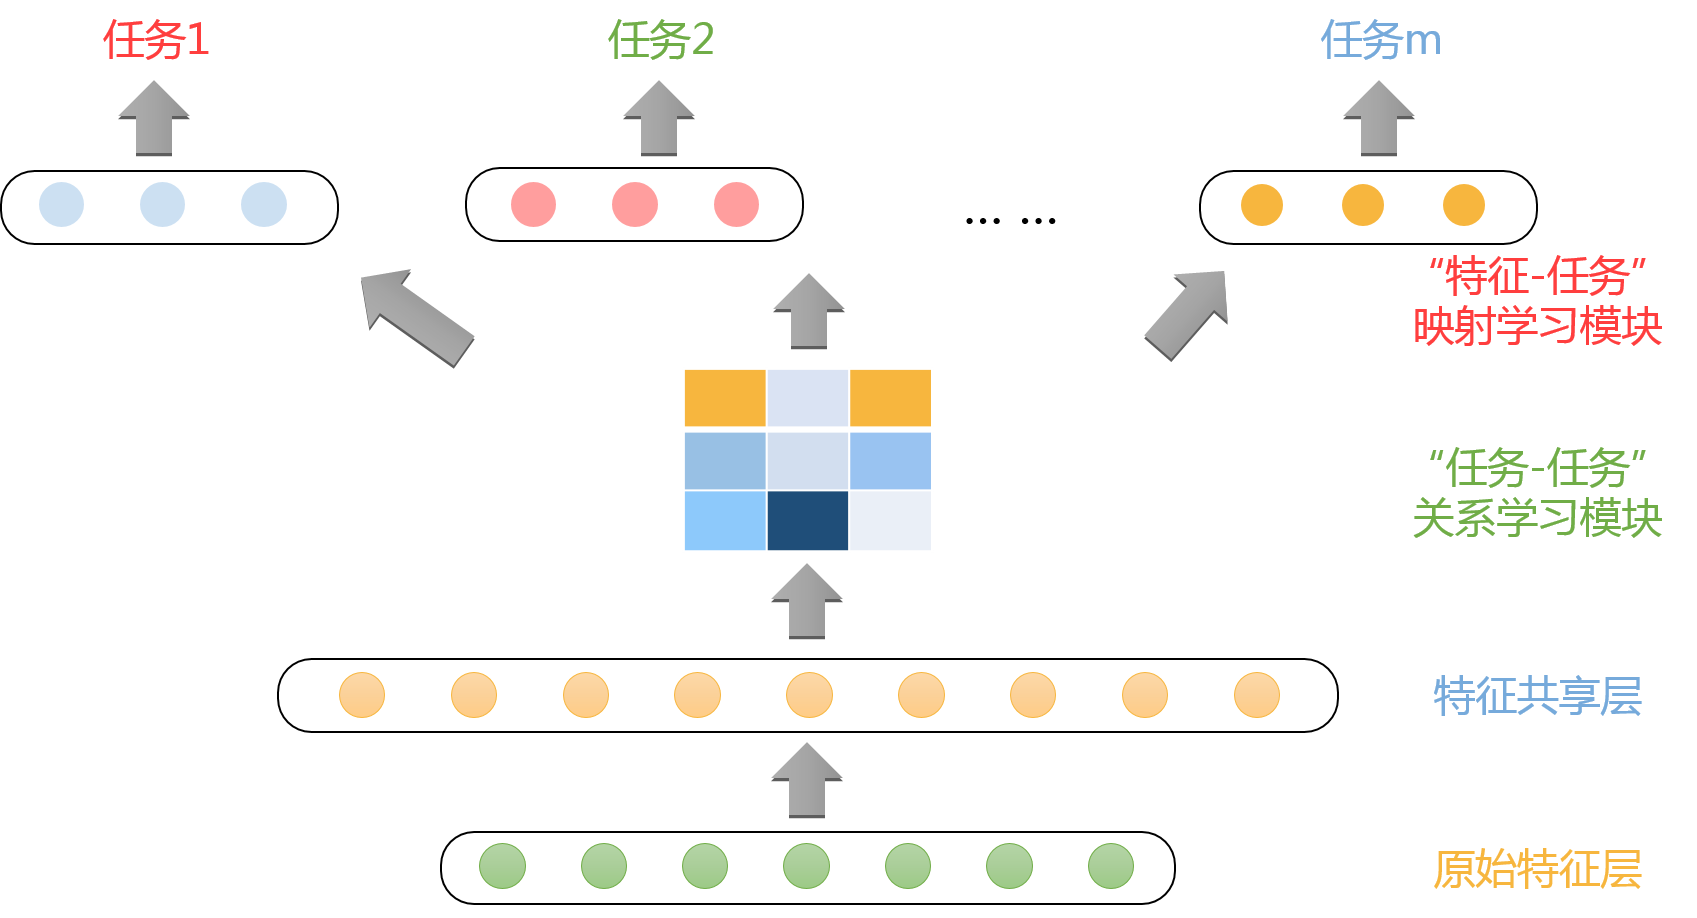
\includegraphics[width=0.8\columnwidth]{figures/multiLearn.png}
	%  \setlength{\abovecaptionskip}{0pt}
	%  \setlength{\belowcaptionskip}{-20pt}
	\caption{多任务学习模型概述}
	\label{MTLmodel}
\end{figure}

目前对深度多任务学习算法的研究所提供的问题解决方案,可以概括地表示为图\ref{MTLmodel}所示的 模型架构,这种结构化的算法可以更好地兼顾不同类别任务之间的层次化结构~\cite{ZhaoQiLu}。与传统的深度卷积神经网络相比,这种深度多任务学习算法能够简化平衡分类器的训练,使得不同种类的评判指标信息可以更好的指导深度神经网络的训练~\cite{DataClassify}。

通过使用这种多指标的联合评估方式,减小了模型不同层之间的训练损失传递,从而更好地提高分类别预测的精确度。


\section{多任务学习模型核心理论}
\subsection{特征提取}
有关商业选址评判的特征提取的理论研究有很多,从大量文献记述中可以总结为从城市维度、商业区维度、商场维度三个层次,来展开的特征提取。在城市维度,现有方法中主要考虑了商场所处的商业区的等级以及功能特性~\cite{cityLevel}。在商业区维度上,则更多地考虑了商业区的商场密度、商业区对顾客的吸引力、商业区内同类型商店所带来的竞争指数以及人流量(通过计算出租车、地铁等dropoff数据来估计)~\cite{traffic}。在最内部的商场维度上,有的研究人员则是从大众点评数据上提取了人均消费、商场大小、促销情况、商场品牌质量(口碑评分)等多种维度的特征~\cite{mallLevel}。将提取的多维度、多种类的特征作为模型的输入进行训练。

此外,还有学者建议将上述指标整合成内部特征与外部特征两类指标进行评价~\cite{IEfeatures}。所谓内部特征,就是指商圈内部对消费者的作用与影响的特征,包括商圈POI数目、商场竞争性与互补性特征等等。而外部特征,则是指商业区周边的环境信息,包括商场周边的人流量数据、交通流量数据以及消费行为分析数据等等,一些典型的特征提取的分类可以用表\ref{feature}所示。

\begin{table}
	\centering
	\caption{内部与外部特征举例}
	\label{feature}
	\begin{tabular}{c|p{8cm}<{\centering}}
	% \begin{tabular}{c|p{8cm}}
		\hline
		\textbf{种类}  & \multicolumn{1}{c}{\textbf{特征实例}}         \\ \hline
		\multirow{6}{*}{内部特征举例} & 店铺平均消费水平 \\ \cline{2-2} 
		                              & 连锁品牌的资产净值 \\ \cline{2-2}
		                              & 商品种类丰富程度   \\ \cline{2-2}
		                              & 连锁店占地面积   \\ \cline{2-2}
		                              & 商圈吸引力指数  \\ \cline{2-2}
									 & 商场竞争力指数   \\ \hline \hline
		\multirow{6}{*}{外部特征举例} & 行人流量密度   \\ \cline{2-2}
									 & 居民区密集度   \\ \cline{2-2}
									 & 地铁节点流量密度   \\ \cline{2-2}
									 & 出租车卸客数   \\ \cline{2-2}
		                             & 易达性       \\ \cline{2-2}
		                             & 周边公交站数目 \\ \hline
	\end{tabular}
\end{table}


\subsection{多任务学习模型}
传统的多任务学习模型主要由4部分组成,包括特征编码层、任务层、关联表征的多任务层和预测层这四个部分~\cite{Caruana1997Multitask,Caruana2012A},我们可以从图\ref{MTLmodel}中看出一种深度多任务学习模型的典型架构图。我们将上一步提取出来的多维度多种类的特征首先需要送入编码层进行编码,对不同类型以及维度的输入特征向量进行线性变换后再通过Relu层,然后送入任务层进行交叉学习,最后通过预测层进行最终的结果预测~\cite{zheng2014urban,Gong2014Efficient}。
\subsubsection{特征编码层}
在这一层中,主要完成对各目标商业区提供的源数据呈现共享表征进行提取,并形成特征向量编码,供下一层的使用~\cite{mariani2018business}。在本层所形成的编码可以表示成如下形式。对于由$n$个连锁店组成的集合$\mathbf{S}$中的每一家连锁店$\mathbf{s_i} \in \mathbf{S}$而言,其内部特征可以表示为
$$\mathbf{x}_i^I = [x_{i,1}^I,x_{i,2}^I,x_{i,3}^I,...,x_{i,D^I}^I]^\mathsf{T} \in R^{D^I}$$
而外部特征则可以用
$$X_i^E = [x_{i,1}^E,x_{i,2}^E,x_{i,3}^E,...,x_{i,D^E}^E]^\mathsf{T} \in R^{D^E}$$
来进行表示~\cite{Wang2018Searchable}。因此,特征编码层的特征向量可以写作
$$\mathbf{x}_i = [\mathbf{x}_i^I;\mathbf{x}_i^E] \in \mathbf{R} ^ D$$
其中$D$表示内部与外部的特征空间$D = D^I + D^E$。
\subsubsection{任务层}
在与任务层相关的研究中,一些研究人员将特征编码层得到的进行编码后特征记为$h_{ENC}$,用公式\ref{taskLayer}描述特定任务层的数学模型
\begin{equation}
	\label{taskLayer}
	c^k=ReLU(W_{TS}^kh_{ENC}+b_{TS}^k)
\end{equation}
其中$b_{TS}^k$是偏置层$(bias)$,$c^k$是将原来的多维多种类特征进行进一步提取得到的降维后任务$k$的新特征~\cite{Held2017Analyzing}。
\subsubsection{关联表征的多任务层}
为了得到不同任务之间的关系,Wang等人的研究工作是在任务层之上引入了一个关系矩阵$R$来表示一个新的关联表征多任务层~\cite{wang2016place}。上层输出的$c^k$ 是第$k$个任务的特征,我们定义在交叉学习$k$个任务之后得到的新的隐藏层特征$\alpha^1,\alpha^2,\alpha^3,\cdots,\alpha^k$的数学模型如下
$$\begin{bmatrix}\alpha^1\\\vdots\\\alpha^k\end{bmatrix}=\begin{bmatrix}R_{11}&\cdots&R_{1K}\\\vdots&\ddots&\vdots\\R_{K1}&\cdots&R_{KK}\end{bmatrix}\cdot\begin{bmatrix}c^1\\\vdots\\c^k\end{bmatrix}$$
在该层的最后,Xu等人通过采用池化(MaxPooling)操作和sigmoid函数操作,将多个任务之间重要的信息特征再次提取出来,得到新的特征$\widetilde c^1\cdots\widetilde c^k$~\cite{xu2016demand,ioffe2015batch}。
\subsubsection{预测层}
预测层是整个多任务学习模型的顶层输出,也是多任务学习的推荐目标。预测层的核心是一个线性变换层,输出$y^k$为相应的预测结果~\cite{Long2017Learning}。
$$y^k=w^k\widetilde c^k+b^k$$
\subsubsection{损失函数}
为了评估模型的预测效果,并对模型进行调整与优化,有必要引入一个合适的损失函数。Jing等人在其相关研究中,考虑使用最小平方损失(least-square loss function)作为多任务学习模型的损失函数进行评估~\cite{Jing2016Where},针对这一类选址问题,这个损失函数可以用公式\ref{loss}表示
\begin{equation}
	\label{loss}
	Loss=\sum_{i=1}^k\sum_{k=1}^K\left\|y_{i_{real}}^k-\;y_i^k\right\|^2\;+\;\mu\;\left\|w\right\|_F^2\;+\;\beta\left\|R\right\|_F^2\;+\;Loss_{ENC}
\end{equation}
损失函数由预测值和真实值的$L2$范数、任务层的参数$W$、多任务之间的关系矩阵$R$以及编码过程产生的Loss这4部分组成。在Golovin等人的实验中,提到了使用Vizier去寻找最优参数的方法~\cite{Golovin2017Google},而在Niu等人的书籍文献中,在优化过程使用加速梯度下降方法AGM(accelerate gradient method),也都产生了比较好的预测效果~\cite{Niu2016Exploiting}。


\subsection{城市商业区划分}
商业区的等级与功能划分,也是商业选址问题中,需要重点考量的因素。同时作为深度多任务学习模型输入的一个维度的评价指标,将为模型的训练提供参考,因此对城市商业区分布的研究便显得尤为重要。这些年以来,地图数据的逐步开源,逐渐带来了着相应的背景数据的开源(又称兴趣点POI)~\cite{feng2015personalized,yin2016adapting}。越来越多的学者想要通过对这些数据的特征来提出一种全新的方法识别商业区以及分类~\cite{wang2015shangyefenji}。
\subsubsection{商业区的识别}
要完成对商业区的划分,首先需要通过一定的指标将商业区的范围进行圈定。参考人们商业活动的习惯,一些研究人员Celikoglu发现,人们的商业活动的基本单位是街区。因而在城市商业区划分问题中,可以选定街区作为基本的划分单位。例如Celikoglu等人将城市按照不同类型的路网分割、进行聚类计算~\cite{celikoglu2016extension}。
\subsubsection{城市商业等级划分}
按照商业活动量的差异,相关研究采用了自然断裂点分类法划分城市的所有商业区为三个等级。划分的主要依据是商业活动量,根据活动量的频率分布直方图,将频率分布突变点作为划分区间端点,划分商业区等级~\cite{li2018ziranduanlie}。
\subsubsection{城市商业功能区划分}
在识别好商业区之后,可以按照一定的指标,参考K-Means聚类算法的相关实现原理,将所有的商业区划分为饮食文化型、专营型、购物中心型、便利型、综合型商业区这五种类型~\cite{frandsen2015automatic}。在这五种类型中,举例来说,饮食文化型商业区聚集了各大餐饮连锁。便利型商业区主要是为周边小区提供生活必需品以及基本生活服务。专营型商业区则是某一类型的商品的贩卖聚集地,常见的有家电电子市场,建材市场等。购物中心型商业区服务类型丰富,服务辐射范围较广。综合型商业区主要包括综合市场、各类专卖店的聚集地等。

\section{实验探究}
针对商业选址这类问题,已有不少学者从多种角度开展了相关实验。以下汇总了使用不同方法,对选址评价指标的预测准确度进行了总结。
\subsection{实验数据准备}
一些学者为了评估关联表征的多任务学习模型在预测精确度上相较于其他方法的优越性,分别采集了以下三个来自北京市的真实数据集进行验证。
大众点评数据:这一数据集主要描述了商业区功能、评级以及评分信息,包含大众点评网上共计456个商场10070家餐饮店以及6028家服饰连锁店的信息~\cite{xia2018dazhongdianping}。
城市交通AFC自助交易记录:在这一实验中,研究人员采集了城市地铁和公交线路乘客的购票记录,采集区间为2017年6月5日至6月17日,共计114232304条数据记录~\cite{huang2018beijingtraffic}。
行车轨迹记录:根据订车平台上以及出租车GPS的行车轨迹记录的数据信息,提取商场周边的人流量信息~\cite{cai2017didi}。
\subsection{评价指标}
为了给出准确性预测,实验随机地将数据集划分训练集和测试集,其中训练集占总数据集规模的60\%,测试集占40\%。对于不同选址模型的评估指标为方均根误差(RMSE)~\cite{fortin2015should}。和皮尔逊相关系数(PCC)。其中,PCC是衡量两个随机变量之间的线性相关性的指标~\cite{schober2018correlation},RMSE指标被广泛的应用于回归误差的分析,其定义如下
$$RMSE\;=\;\sqrt{\frac{{\displaystyle\sum_{i=1}^k}{\displaystyle\sum_{k=1}^K}\left(y_i^k\;-\;\widehat y_i^k\right)^2}{nK}}$$
\subsection{实验应用方法}
实验中所采用的方法如表\ref{tb:exp-method}中所示。

\begin{table}[]
	\centering
	\caption{实验方法列表}
	\label{tb:exp-method}
	\begin{tabular}{|c|l|}
		\hline
		方法名称                               & \multicolumn{1}{c|}{方法描述}                                                                                      \\ \hline
		RF                                 & \begin{tabular}[c]{@{}l@{}}随机森林(Random Forest)是一种\\ 利用多棵树对样本进行训练和预测的一种分类器,\\ 实验中选择的随机森林的树的数量为60棵。\end{tabular} \\ \hline
		\multicolumn{1}{|l|}{Cross-Stitch} & \begin{tabular}[c]{@{}l@{}}一种通过Cross-stitch单元\\ 来共享两个任务之间信息的\\ 深度多任务学习方法~\cite{misra2016cross}。\end{tabular}                         \\ \hline
		DT                                 & \begin{tabular}[c]{@{}l@{}}决策树(Decision Tree)是一种常用的\\ 树形结构分类方法\\ 在实验中约定树的最大深度为2。\end{tabular}                  \\ \hline
		KNN-unif                           & \begin{tabular}[c]{@{}l@{}}这种方法通过联合权重\\ 训练一个回归模型\\ 在实验中为KNN网络使用6个最近邻的邻居节点。\end{tabular}                        \\ \hline
	\end{tabular}
\end{table}

\subsection{实验结果分析}
表\ref{tb:RMSEcanyin}和表\ref{tb:RMSEfushi}的实验结果,分别展现了采用关联特征的深度多任务学习模型(Deep Multi-task Learning framework with Relational Attention, DMLRA),和其他传统模型,在餐饮和服饰两个数据集上的预测结果的RMSE指标。

\begin{table}[!hpt]
	\centering
	\caption{基于餐饮连锁店数据集的各种预测方法的RMSE指标}
	\label{tb:RMSEcanyin}
	\begin{tabular}{p{2cm}<{\centering}p{2cm}<{\centering}p{2cm}<{\centering}p{2cm}<{\centering}p{2cm}<{\centering}p{2cm}<{\centering}}
		\hline
		& \textbf{y1} & \textbf{y2} & \textbf{y3} & \textbf{y4} & \textbf{y4} \\ \hline
		RF & 1156.625 & 3.921 & 0.518 & 0.521 & 0.567 \\ %\hline
		DT & 1278.090 & 4.109 & 0.543 & 0.581 & 0.604 \\ %\hline
		Cross-Stitch & 1068.238 & 3.744 & 0.533 & 0.494 & 0.540 \\ \hline
		\textbf{DMLRA} & \textbf{933.406} & \textbf{3.611} & \textbf{0.488} & \textbf{0.479} & \textbf{0.536}                 \\ \hline
	\end{tabular}
\end{table}

首先,随机森林、决策树等传统的单一任务学习方法和cross-stitch这种多任务学习方法更多的依赖于任务关系假设,这就导致了这些方法相比于深度多任务学习模型而言灵活度更低。观测数据显示,DMLRA可以更有效地实现正负样本转换控制的自适应。

\begin{table}[!hpt]
	\centering
	\caption{基于服饰连锁品牌数据集的各种预测方法的RMSE指标}
	\label{tb:RMSEfushi}
	\begin{tabular}{p{2cm}<{\centering}p{2cm}<{\centering}p{2cm}<{\centering}p{2cm}<{\centering}p{2cm}<{\centering}p{2cm}<{\centering}}
		\hline
		& \textbf{y1} & \textbf{y2} & \textbf{y3} & \textbf{y4} & \textbf{y4} \\ \hline
		RF & 33.555 & 3.149 & 0.439 & 0.439 & 0.459 \\ %\hline
		DT & 53.900 & 3.319 & 0.475 & 0.477 & 0.468 \\ %\hline
		Cross-Stitch & 29.845 & 2.818 & 0.399 & 0.404 & 0.416 \\ \hline
		\textbf{DMLRA} & \textbf{23.287} & \textbf{2.668} & \textbf{0.361} & \textbf{0.386} & \textbf{0.397}                 \\ \hline
	\end{tabular}
\end{table}

其次,可以从实验结果中注意到,采用了DMLRA模型的方法进行预测可以在大多数任务上,取得显著更优的RMSE和PCC指标。


\section{结论}
本文综述了为连锁品牌新店选址进行推荐的方法。首先从商圈的特征提取入手,将与选址评判相关的因素,整合成内部与外部两类特征,作为深度多任务学习模型的输入。其次,在论述传统的多任务学习方法的基础上,目前新提出的基于关联特征的深度多任务学习方法,能够自适应地控制正负样本之间的转换。特别地,该方法引入了一种特殊任务追踪机制来为不同的学习任务指定特征,因为商业选址成功性判定的准则依赖于共享特征集上的不同维度。另外,该方法还设计了一个关联学习模型来区分多重准则之间的联系。为了评估模型的效果,本文引用了部分学者在真实数据集的基础上,开展的大量实验,并分别与传统方法和目前最先进的方法进行验证,以给出性能指标评价结果。实验结果显示,基于关联特征的深度多任务学习模型的实现效果,在一定程度上优于传统方法的实现效果。


\subsubsection*{致谢}
首先要感谢软件国家重点实验室杜博文与孙磊磊两位老师,对我完成本篇文献综述过程中所提供的指导。此外还要感谢荣文戈老师以及我身边的同学,对我在使用文本编辑工具方面提供的帮助。最后要感谢家人和朋友一直以来的支持与关爱。

\bibliographystyle{splncs03}
%\bibliographystyle{unsrt}
\bibliography{reference}
	
\end{document}
